\documentclass{article}

\usepackage[english]{babel}

% Set page size and margins
\usepackage[a4paper,top=2cm,bottom=2cm,left=3cm,right=3cm,marginparwidth=1.75cm]{geometry}

% Useful packages
\usepackage{amsmath}
\usepackage{graphicx}
\usepackage[colorlinks=true, allcolors=blue]{hyperref}
\usepackage{color}


\title{Your Title goes here}
\author{2100816}
\begin{document}
\maketitle

\begin{table}[h]
    \centering
    \begin{tabular}{ll}
        Registration number: & \textcolor{red}{2100816}\\
        Project: & \textcolor{red}{Causal inference}\\
        Link to GitHub: & \url{https://github.com/11BelowStudio/ce888}\\
    \end{tabular}
\end{table}



\begin{table}[h]
    \centering
    \begin{tabular}{lc}
        Executive summary (max.\ 250 words) & \textcolor{red}{Your word count}\\
        Introduction (max.\ 600 words) & \textcolor{red}{Your word count}\\
        Data (max.\ 500 words/dataset) & \textcolor{red}{Your word count}\\
        Methodology (max.\ 600 words) & \textcolor{red}{Your word count}\\
        Conclusions (max.\ 500 words) & \textcolor{red}{Your word count}\\
        \hline
        Total word count & \textcolor{red}{Your word count}\\
    \end{tabular}
    %\caption{Word counts for each section.}
\end{table}

\tableofcontents

\clearpage



\begin{abstract}
Your executive summary goes here.
\end{abstract}


\section{Introduction}

Your introduction goes here! Simply start writing your document and use the
Recompile button to view the updated PDF preview.

Examples of commonly used commands and features are listed below, in
Section~\ref{sec:tutorial}, to help you get started.
Instructions on what to include in each section are given in the assignment description

\href{https://moodle.essex.ac.uk/draftfile.php/196919/user/draft/666046553/2021_CE888_Assignment_1.pdf}{here}.

\section{Data}

This project involves two datasets: IHDP\cite{Gross1993}\cite{BROOKSGUNN1992350} and JOBS\cite{JOBS_LaLonde}.

\subsection{IHDP - The Infant Health Development Program}

* premature infants

* x: measurements taken when the kid was born, along with info about the home situation/what the mother was doing during pregnancy

* y: IQ test results

This dataset contains factual and counterfactual data.

\begin{figure}[tb]
\centering
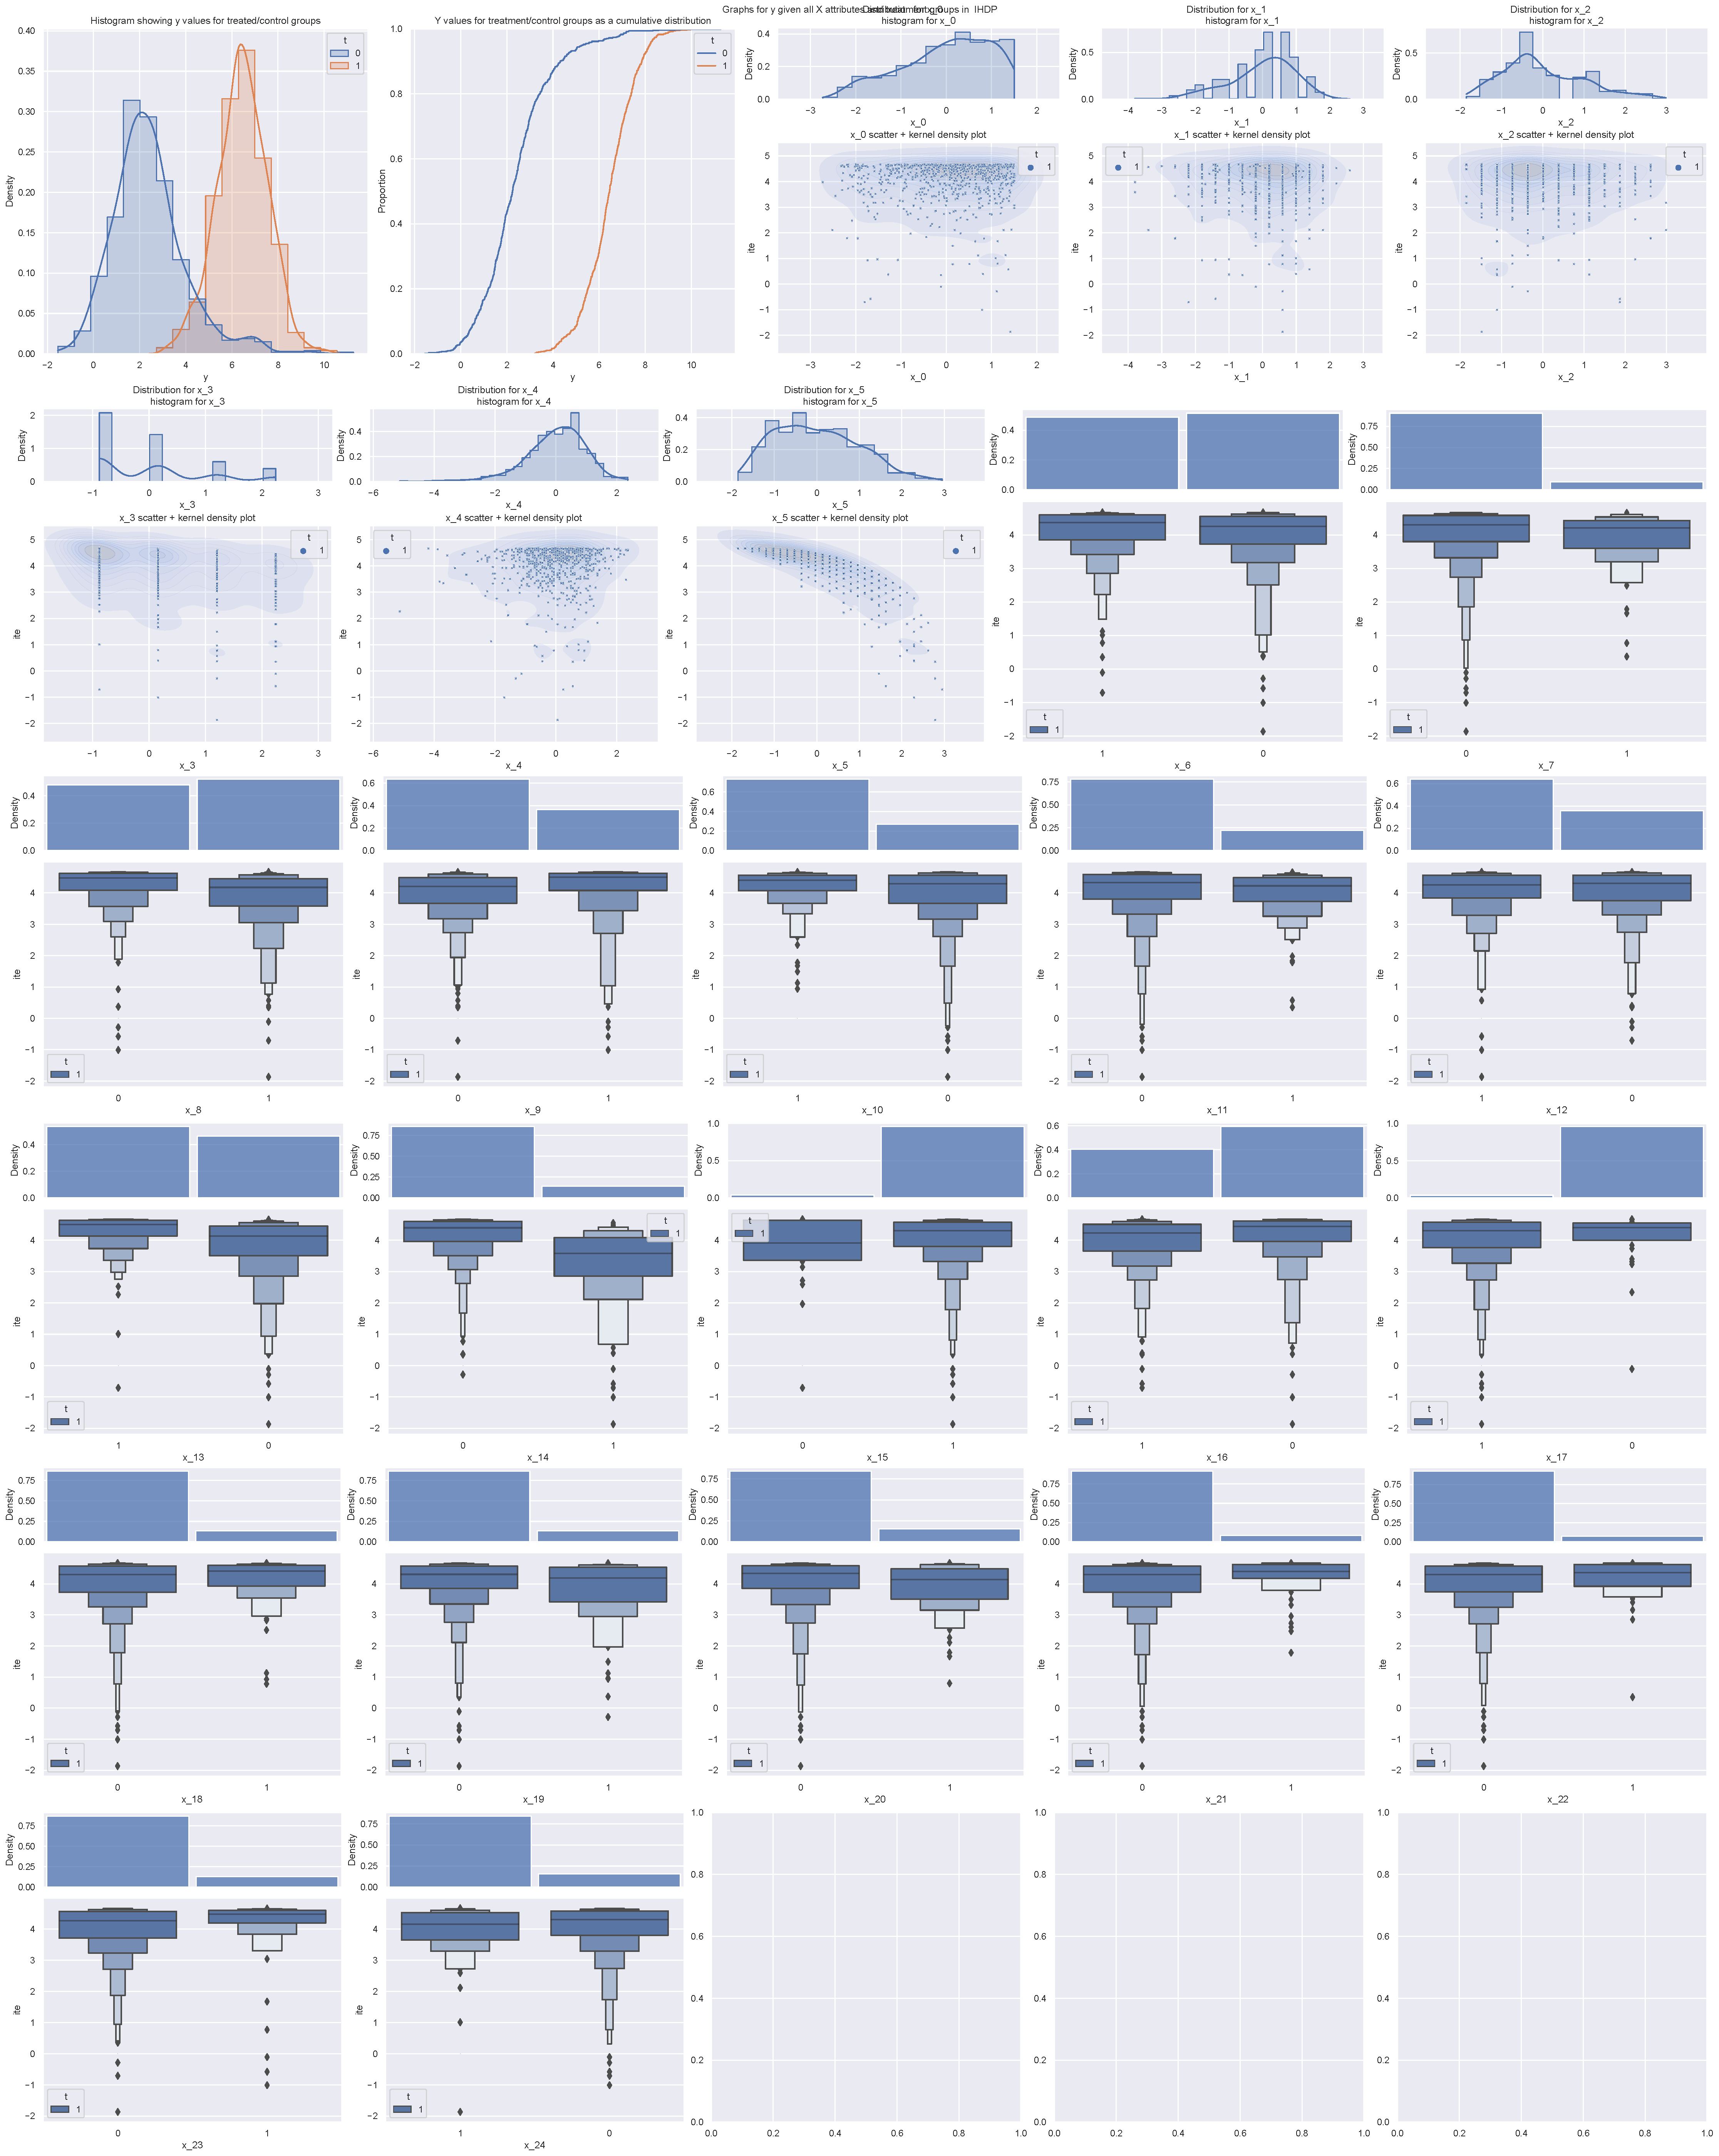
\includegraphics[width=1\textwidth]{project/data/ihdp_graphs.pdf}
\caption{\label{fig:ihdpgraphs}Several graphs for the IHDP dataset}
\end{figure}


\begin{figure}[tb]
\centering
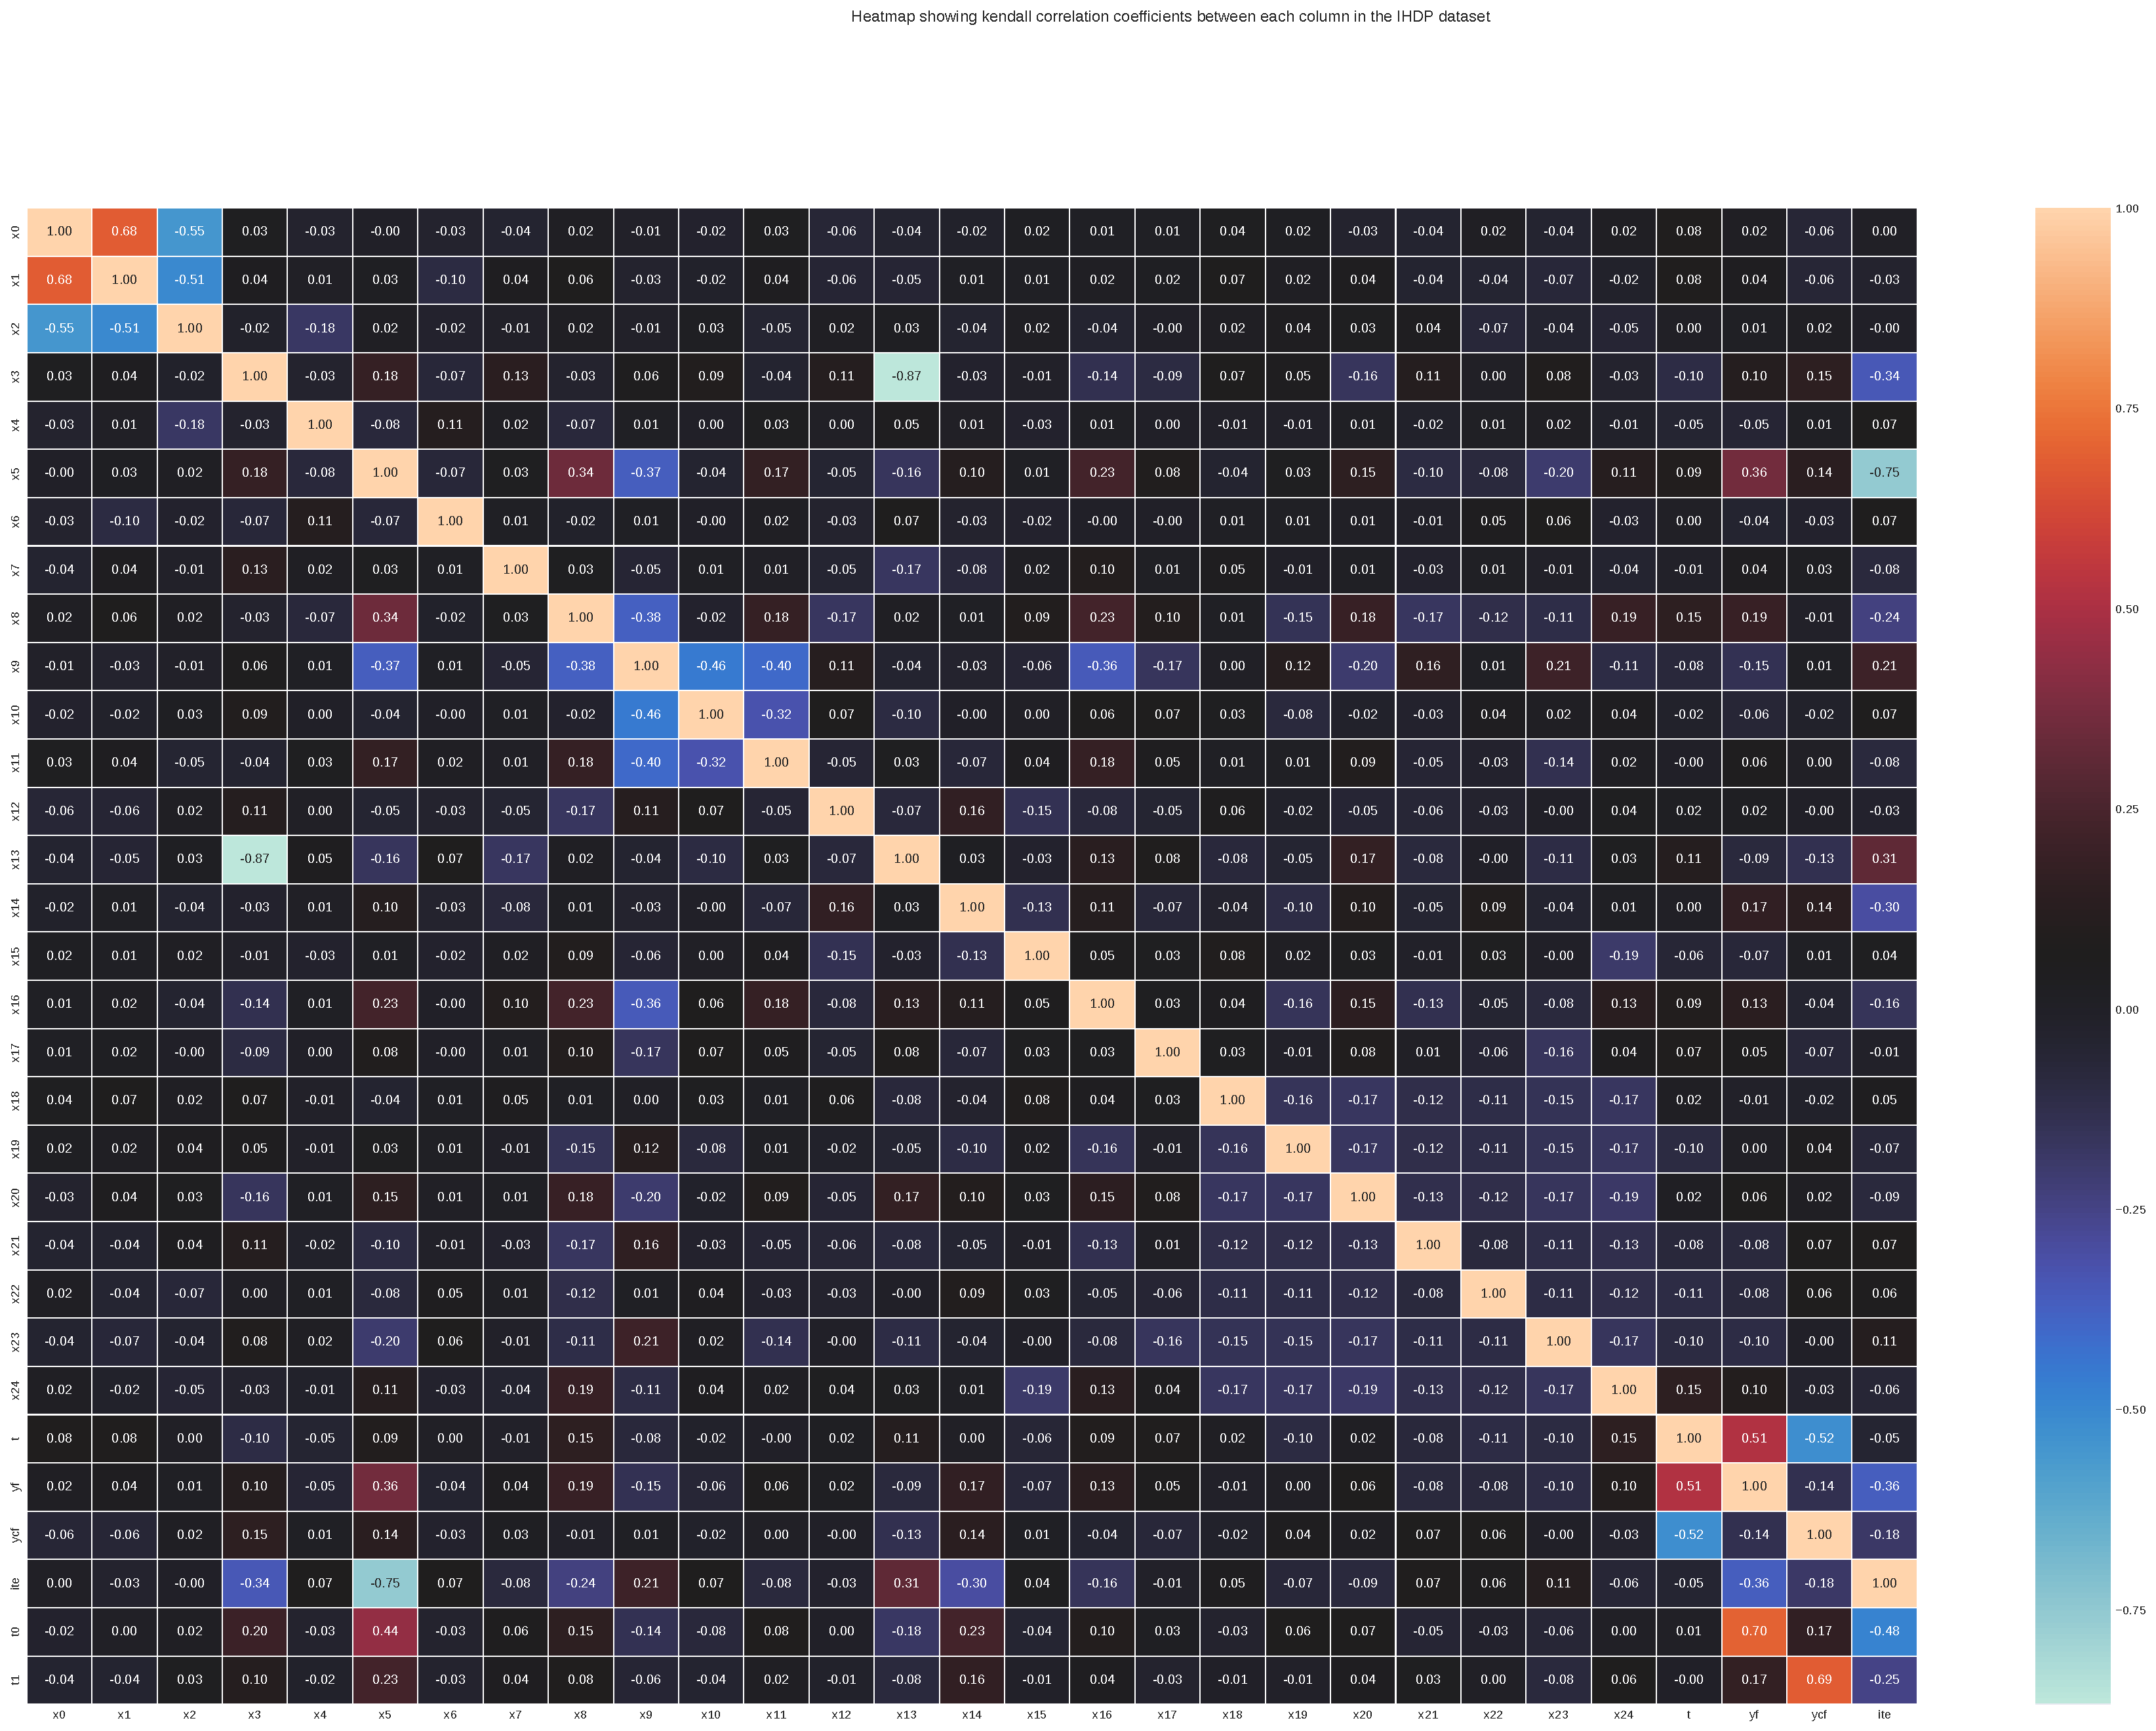
\includegraphics[width=1\textwidth]{project/data/ihdp_heatmap.pdf}
\caption{\label{fig:ihdp_correlation}Correlation heatmap for the IHDP dataset}
\end{figure}



\subsection{JOBS}

\begin{figure}[tb]
\centering
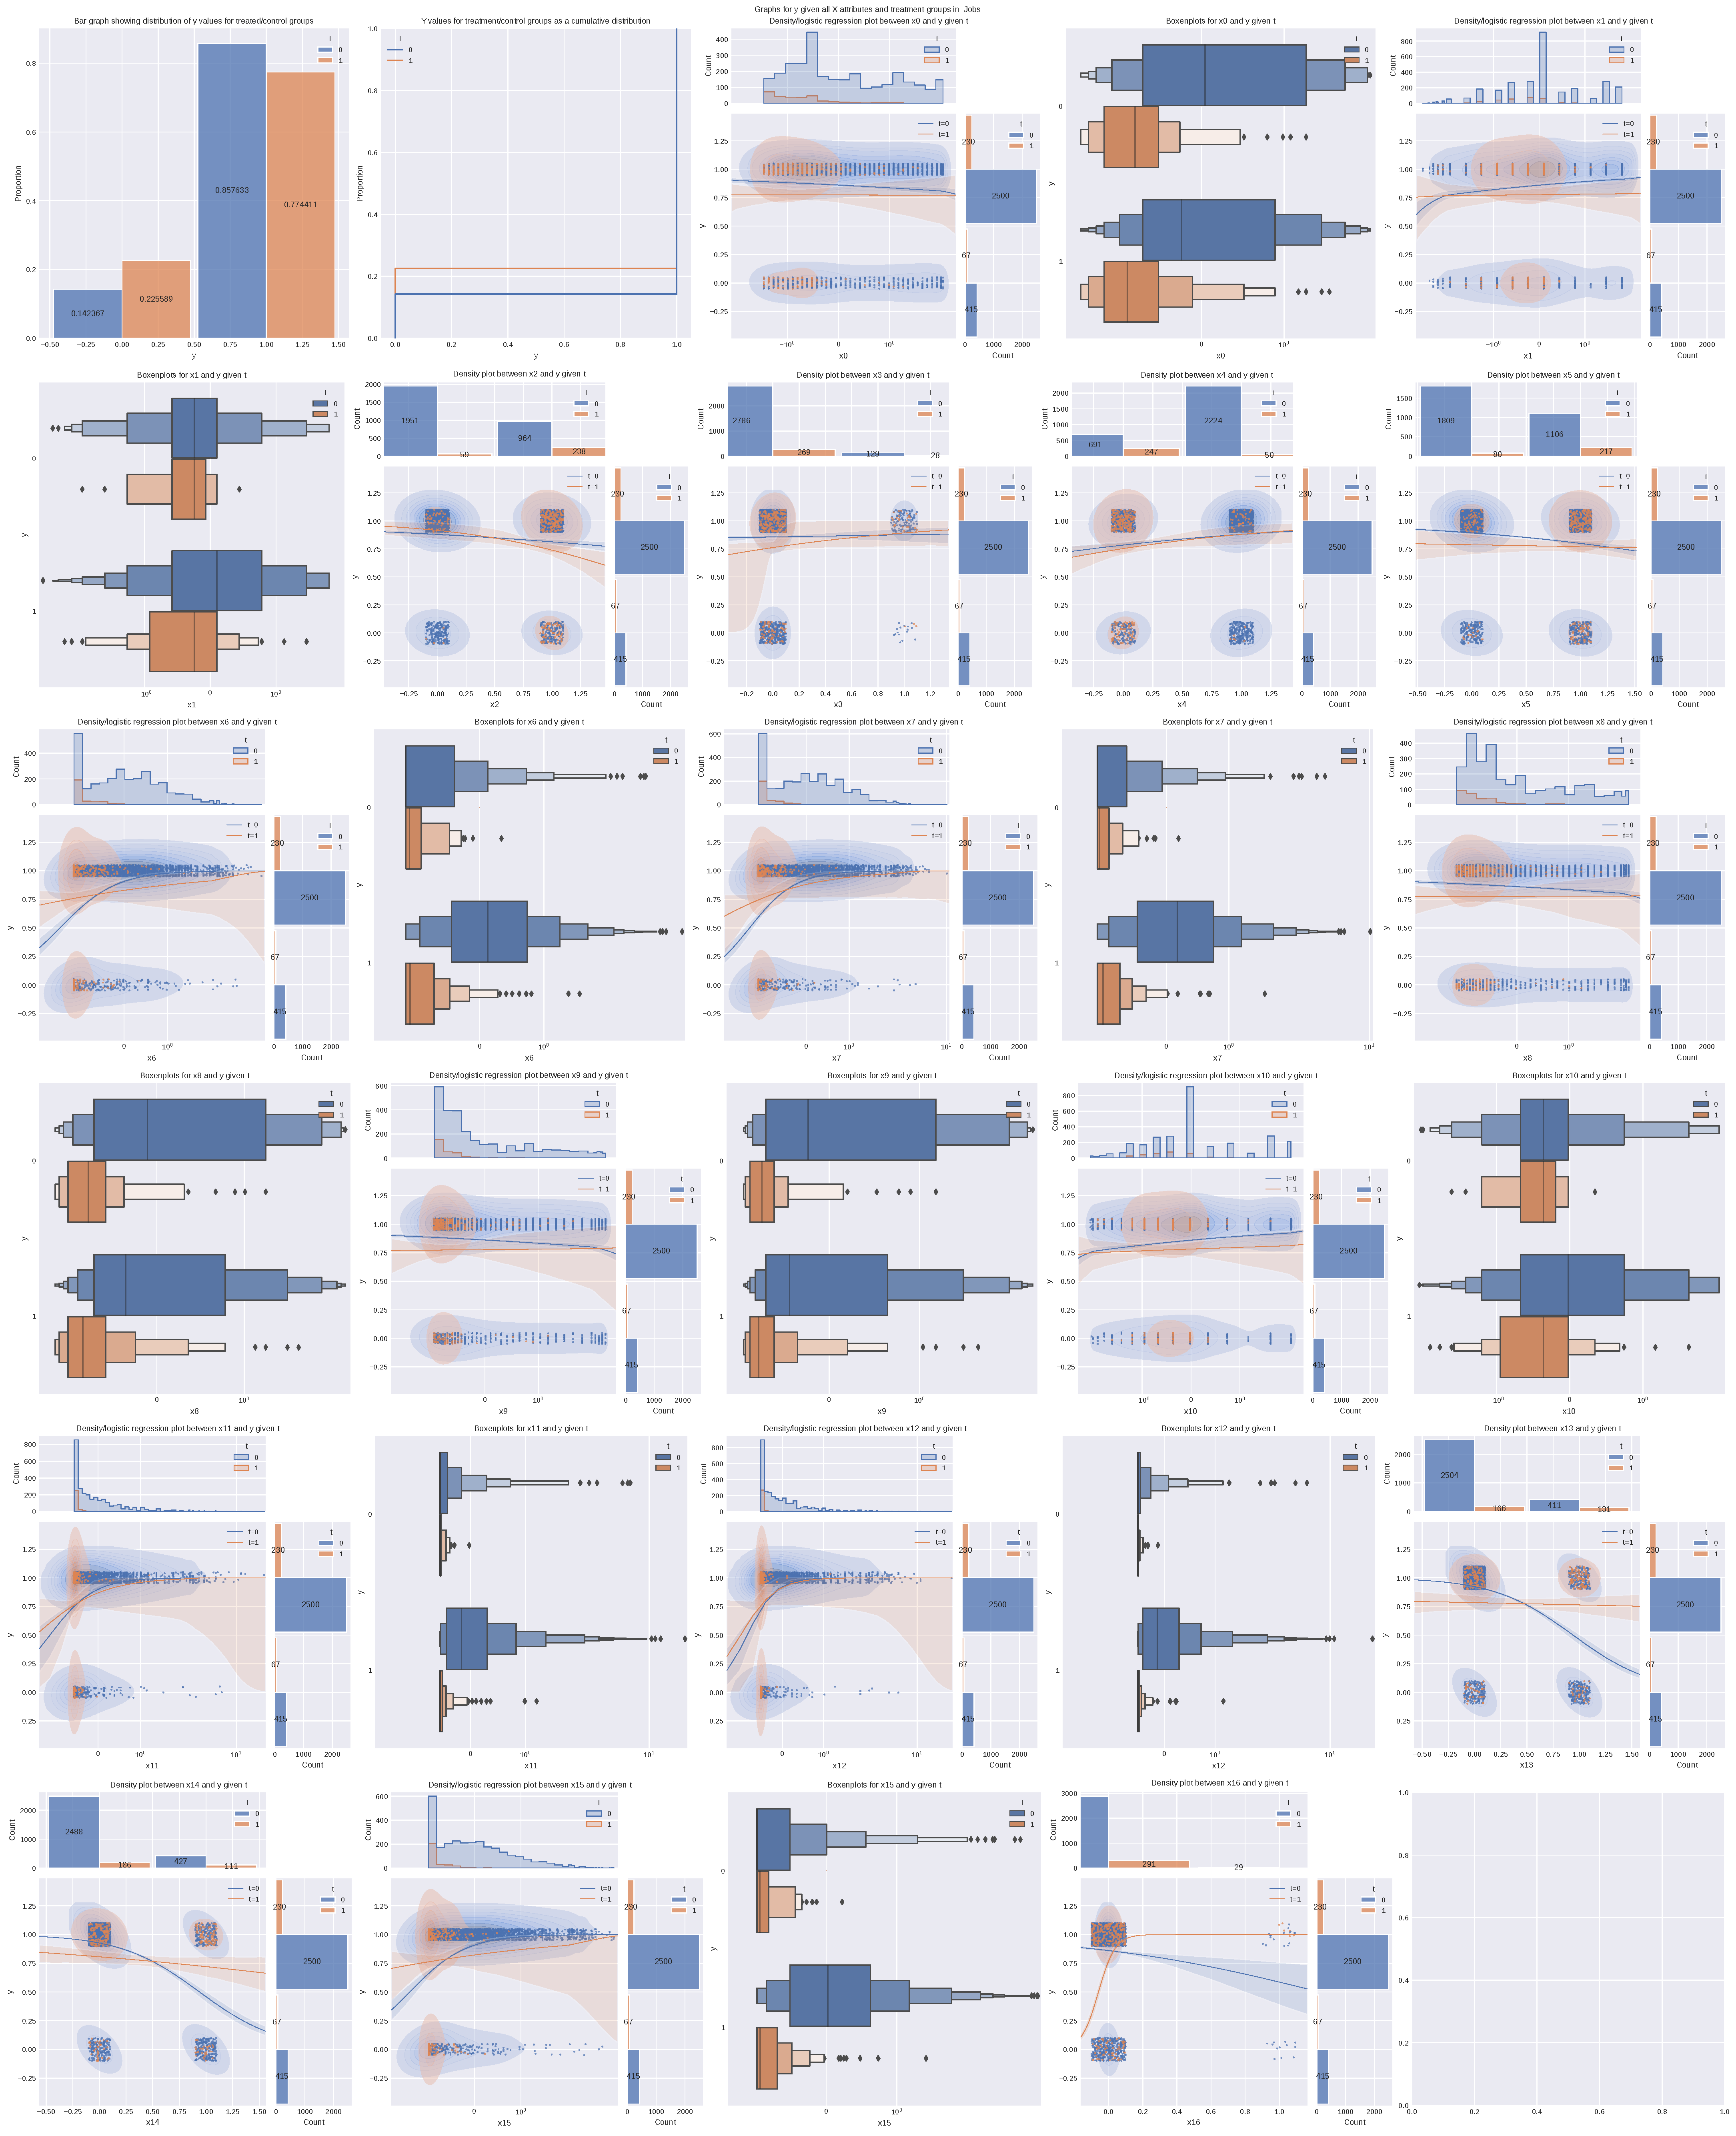
\includegraphics[width=1\textwidth]{project/data/jobs_graphs.pdf}
\caption{\label{fig:jobsgraphs}Several graphs for the JOBS dataset}
\end{figure}


\begin{figure}[tb]
\centering
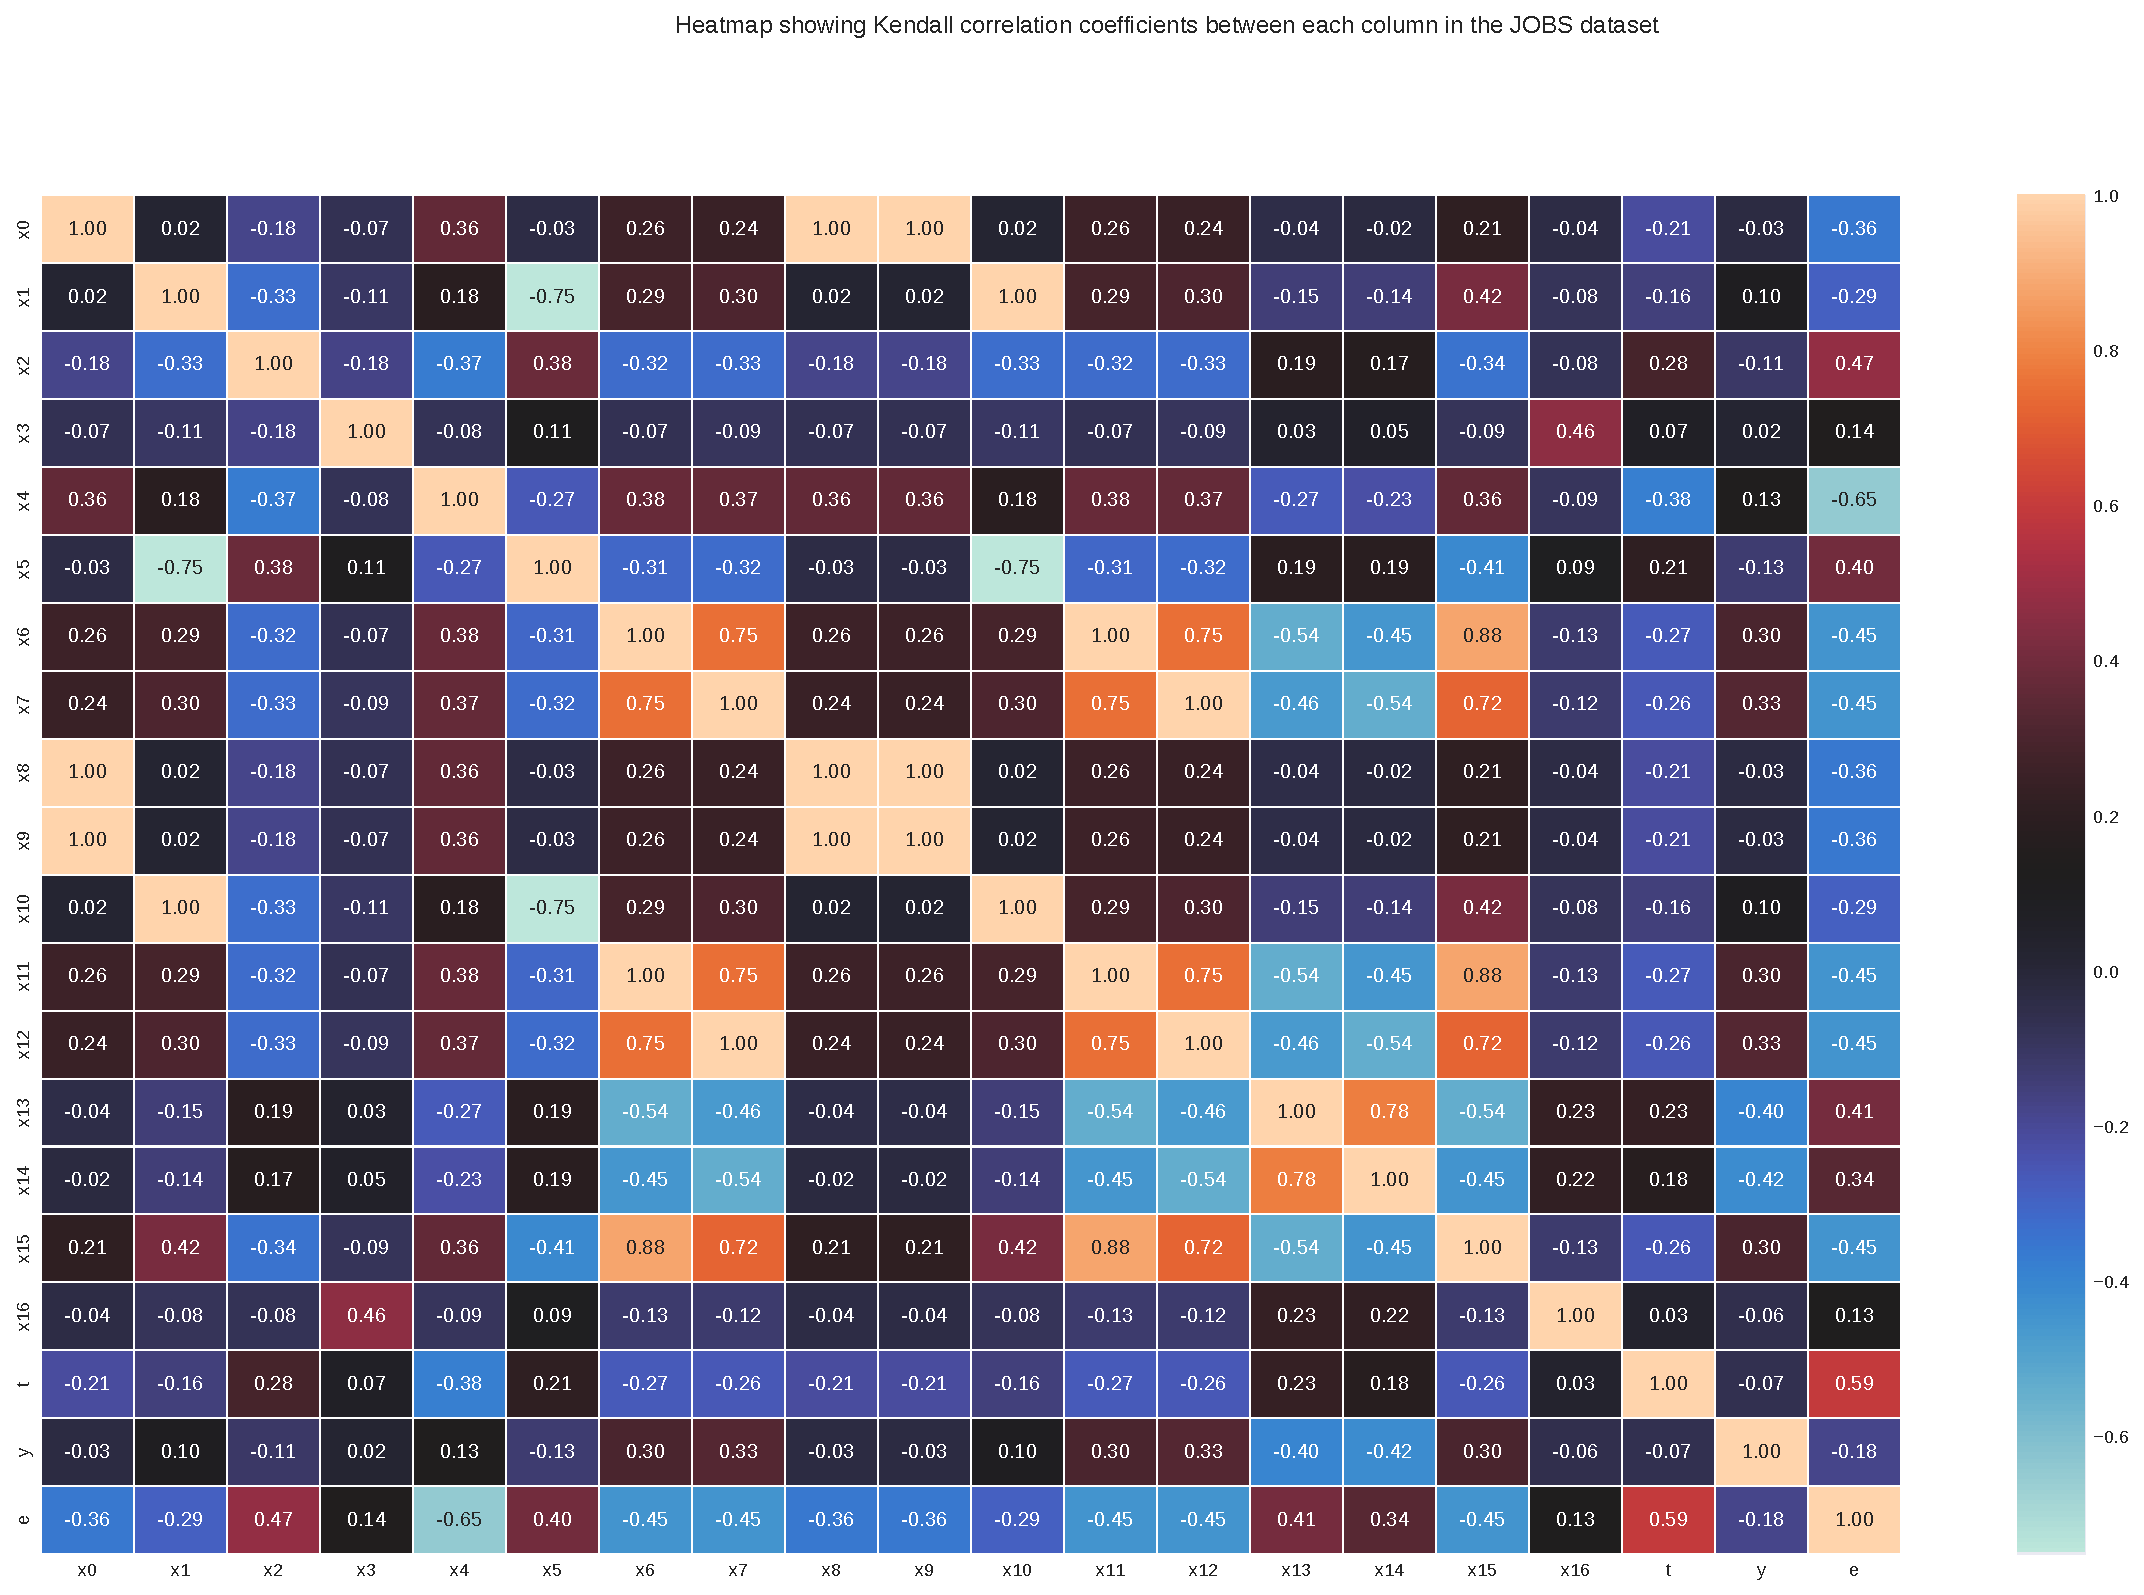
\includegraphics[width=1\textwidth]{project/data/jobs_heatmap.pdf}
\caption{\label{fig:jobs_correlation}Correlation heatmap for the JOBS dataset}
\end{figure}



If you have only one dataset to work on, there is no need to add subsections to this section.
Otherwise, simply use the subsection command as shown in the tutorial below to create
separate subsections for each of the datasets.

The title of the subsection should be representative of the dataset (and not ``Dataset 1/2/3'').

Make sure you properly cite the origin of the dataset/s.

\section{Methodology}

Add subsections as needed.

\section{Conclusions}

Should not include subsections.

From here (included) to line 139, there is a tutorial for you to learn how to add tables,
figures, create subsections, etc.
You should delete all of that after reading it, and not submit it as part of your report.

\section{Latex Tutorial}
\label{sec:tutorial}

To get the word count per section, you can use: \url{https://app.uio.no/ifi/texcount/online.php}

This section is only for you to learn how to write in LateX. Delete it after reading it.


\subsection{How to include Figures}

First you have to upload the image file from your computer using the upload link in the file-tree menu.
Then use the include graphics command to include it in your document.
Use the figure environment and the caption command to add a number and a caption to your figure.
See the code for Figure \ref{fig:frog} in this section for an example. Include the code for figures
and tables directly after the paragraph where you reference them.

\begin{figure}[tb]
\centering
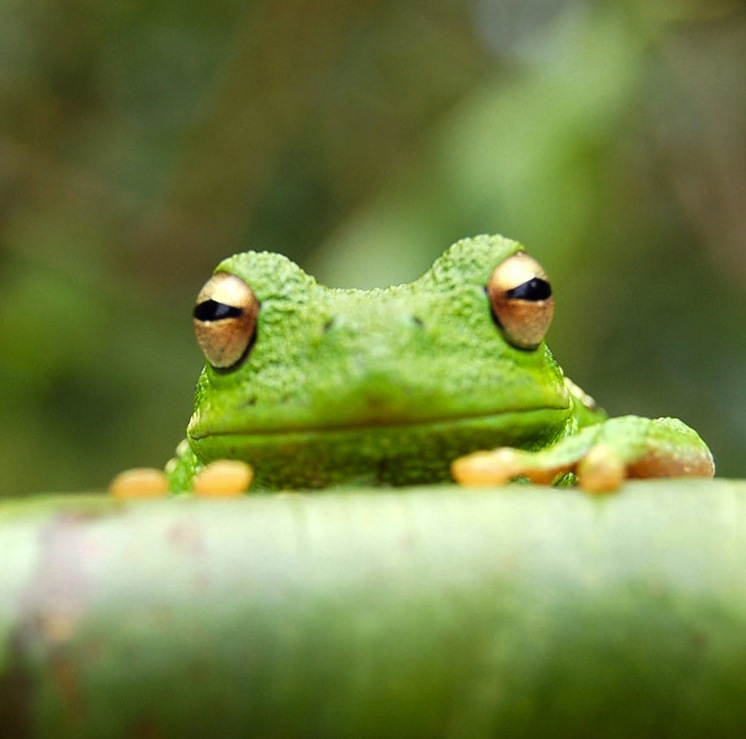
\includegraphics[width=0.3\textwidth]{frog.jpg}
\caption{\label{fig:frog}This frog was uploaded via the file-tree menu.}
\end{figure}

Note that your figure will automatically be placed in the most appropriate place for it,
given the surrounding text and taking into account other figures or tables that may be close by
(which is waaaay nicer than doing it on Word!).
You can find out more about adding images to your documents in this help article on
\href{https://www.overleaf.com/learn/how-to/Including_images_on_Overleaf}{including images on Overleaf}.



\subsection{How to add Tables}

Use the table and tabular environments for basic tables --- see Table~\ref{tab:widgets}.
For more information, please see this help article on \href{https://www.overleaf.com/learn/latex/tables}{tables}.

\begin{table}[tb]
\centering
\begin{tabular}{l|r}
Item & Quantity \\\hline
Widgets & 42 \\
Gadgets & 13
\end{tabular}
\caption{\label{tab:widgets}An example table.}
\end{table}


\subsection{How to add Lists}

You can make lists with automatic numbering \dots

\begin{enumerate}
\item Like this,
\item and like this.
\end{enumerate}
\dots or bullet points \dots
\begin{itemize}
\item Like this,
\item and like this.
\end{itemize}

\subsection{How to write Mathematics}

\LaTeX{} is great at typesetting mathematics. Let $X_1, X_2, \ldots, X_n$ be a sequence of independent and identically distributed random variables with $\text{E}[X_i] = \mu$ and $\text{Var}[X_i] = \sigma^2 < \infty$, and let
\[S_n = \frac{X_1 + X_2 + \cdots + X_n}{n}
      = \frac{1}{n}\sum_{i}^{n} X_i\]
denote their mean. Then as $n$ approaches infinity, the random variables $\sqrt{n}(S_n - \mu)$ converge in distribution to a normal $\mathcal{N}(0, \sigma^2)$.


\subsection{How to add Citations and a References List}

You can simply upload a \verb|.bib| file containing your BibTeX entries, created with a tool such as JabRef. You can then cite entries from it, like this: \cite{greenwade93}. Just remember to specify a bibliography style, as well as the filename of the \verb|.bib|. You can find a \href{https://www.overleaf.com/help/97-how-to-include-a-bibliography-using-bibtex}{video tutorial here} to learn more about BibTeX.


\bibliographystyle{abbrv}
\bibliography{sample}

\end{document}